
\section{Microsoft SQL Server}
\label{part:sql-server}

Microsoft SQL Server is one of the most widely deployed data management platforms in the enterprise. It combines relational database, data warehousing, business intelligence, and advanced analytics into a single coherent ecosystem, available both on-premises and in the Azure cloud.

\subsection{Editions and Licensing}
\label{sec:sql-server-editions}

SQL Server ships in several editions, each designed for a different combination of scale, feature set, and budget:

\begin{notebox}
\textbf{Enterprise}: aimed at mission-critical workloads. It offers advanced capabilities: in-memory OLTP, compression, unlimited partitioning, Always On for high availability, and integrated analytics. It imposes no hardware resource limits.

\textbf{Standard}: the core data management and business intelligence features. Its limits are 128 GB of RAM for the buffer pool and 24 cores. It suits departmental workloads and mid-tier applications.

\textbf{Express}: the free entry-level version. Its limits are 10 GB of storage per database, 1 GB of RAM, and 4 cores. It suits desktop applications, prototypes, and small servers.

\textbf{Developer}: a full replica of the Enterprise edition, free for development and testing only. It cannot be used in production.
\end{notebox}

The cloud editions (Azure SQL Database, Azure SQL Managed Instance) offer pay-as-you-go pricing with elastic scaling.

\subsection{Architecture of the Suite}
\label{sec:sql-server-architecture}

The SQL Server ecosystem groups specialized components that span the entire business intelligence stack:

{
\scriptsize
\begin{center}
\begin{tabular}{@{}lll@{}}
\toprule
\textbf{Function} & \textbf{On-premises} & \textbf{Cloud / Self-service} \\
\midrule
Database Engine & SQL Server & Azure SQL Database \\
Data integration & SSIS & Azure Data Factory, Power Query \\
OLAP analysis & SSAS & Azure Analysis Services, Power Pivot \\
Reporting & SSRS & Power BI, Paginated Reports \\
Data Quality & DQS & --- \\
Master Data & MDS & --- \\
\bottomrule
\end{tabular}
\end{center}
}

\subsubsection{Core Components}
\label{subsec:sql-server-components}

\begin{itemize}
    \item \textbf{SQL Server Database Engine}: the core relational engine that manages storage, query processing, transactions, and security.

    \item \textbf{SQL Server Integration Services (SSIS)}: a platform for orchestrating ETL flows and moving data between heterogeneous sources (see Part~\ref{part:etl-ssis}).

    \item \textbf{SQL Server Analysis Services (SSAS)}: an engine for multidimensional OLAP processing (cubes) and in-memory tabular models (see Part~\ref{part:ssas}).

    \item \textbf{SQL Server Reporting Services (SSRS)}: a platform for creating, managing, and distributing structured, paginated reports.

    \item \textbf{Master Data Services (MDS)}: a solution for centrally managing an organization's master data (customers, products, hierarchies), guaranteeing a ``single version of truth''.

    \item \textbf{Data Quality Services (DQS)}: tools for knowledge-driven data cleansing and matching.
\end{itemize}

\subsubsection{Development and Administration Tools}
\label{subsec:sql-server-tools}

\textbf{SQL Server Management Studio (SSMS)}: an integrated environment for administration and development. It connects to every component of the platform (Database Engine, Analysis Services, Integration Services, Reporting Services). Its main features are the Object Explorer for navigating objects, the Query Editor with IntelliSense, the Activity Monitor for tuning, and backup/restore tools.

\textbf{SQL Server Data Tools (SSDT)}: an extension of Visual Studio for developing database projects (schema, stored procedures, deployment), SSIS packages, SSAS models, and SSRS reports. It supports source control and CI/CD.

\textbf{Azure Data Studio}: a lightweight cross-platform editor optimized for queries and notebooks. It is extensible through plugins for PostgreSQL, Kubernetes, and others.

\begin{theorybox}[frametitle={Resources}]
\textbf{Official documentation}: \url{https://docs.microsoft.com/sql}

\textbf{Learn}: \url{https://docs.microsoft.com/learn/paths/get-started-querying-with-transact-sql}
\end{theorybox}

\subsection{System Databases}
\label{sec:system-databases}

SQL Server maintains four system databases that the instance needs to run. They are created automatically during installation and must never be deleted.

\begin{examplebox}
\textbf{master}: the central catalog of the instance. It holds metadata on every user database, logins and credentials, server configurations, linked servers, and endpoints. Its integrity is critical: if \texttt{master} is corrupted, the instance does not start. It requires regular backups.

\textbf{model}: the template for creating new databases. Any change to \texttt{model} (options, filegroups, objects) propagates automatically to databases created afterward, which helps standardize organization-wide configurations.

\textbf{msdb}: hosts the metadata of SQL Server Agent: scheduled jobs, alerts, operators, and execution history. It also holds SSIS packages deployed in the legacy Package Store and the Database Mail configuration.

\textbf{tempdb}: a temporary database recreated at every instance restart (it does not persist). It serves local temporary tables (\texttt{\#temp}) and global ones (\texttt{\#\#temp}), table variables, cursors, sort and hash operations that spill out of memory, and the version store for snapshot isolation. Its performance affects the whole server.
\end{examplebox}

\subsection{Namespace and Object Identification}
\label{sec:sql-server-namespace}

\subsubsection{Name Hierarchy}
\label{subsec:naming-hierarchy}

SQL Server organizes objects along a four-level hierarchy:

\begin{center}
\texttt{[server.][database.][schema.]object}
\end{center}

\begin{itemize}
    \item \textbf{Server}: the SQL Server instance (relevant for linked servers and distributed queries).
    \item \textbf{Database}: a logical container of objects. Every connection has a current database.
    \item \textbf{Schema}: a namespace inside the database that groups related objects. The default schema is \texttt{dbo} (database owner).
    \item \textbf{Object}: a table, view, stored procedure, function, and so on.
\end{itemize}

\subsubsection{Name Resolution}
\label{subsec:name-resolution}

When parts of a name are omitted, SQL Server applies default values:

\begin{lstlisting}
-- Use current database, user's default schema
SELECT * FROM customers

-- Specify the schema explicitly
SELECT * FROM dbo.customers

-- Specify database and schema
SELECT * FROM sales_db.dbo.customers

-- Fully qualified name (for linked server)
SELECT * FROM REMOTE_SERVER.sales_db.dbo.customers
\end{lstlisting}

\begin{notebox}
\textbf{Best practice.}
Always qualifying objects with their schema (\texttt{dbo.table}) improves performance (it avoids the lookup in the user's schema) and prevents ambiguity when objects of the same name exist in different schemas.
\end{notebox}

\subsection{Data Import and Export}
\label{sec:import-export}

\subsubsection{Import/Export Wizard}
\label{subsec:import-export-wizard}

Management Studio provides a graphical wizard to transfer data between heterogeneous sources. It is reached by right-clicking the database $\rightarrow$ \texttt{Tasks} $\rightarrow$ \texttt{Import Data} or \texttt{Export Data}.

Internally the wizard generates an SSIS package that can either run immediately or be saved for reuse. The supported sources and destinations include flat files (CSV, fixed-width), Excel, Access, OLE DB providers, ODBC connections, and other SQL Server databases.

\subsubsection{Bulk Insert}
\label{subsec:bulk-insert}

For massive loads from files, the \texttt{BULK INSERT} command outperforms the wizard:

\begin{lstlisting}
BULK INSERT dbo.customers
FROM 'C:\data\customers.csv'
WITH (
    FIELDTERMINATOR = ',',
    ROWTERMINATOR = '\n',
    FIRSTROW = 2  -- Skip header
);
\end{lstlisting}

The command-line utility \texttt{bcp} (Bulk Copy Program) offers similar functionality with greater flexibility.

\subsubsection{XML Export with FOR XML}
\label{subsec:for-xml}

SQL Server supports native XML output through the \texttt{FOR XML} clause, with several formatting modes:

\textbf{RAW}: each row becomes a \texttt{<row>} element with its columns as attributes.
\begin{lstlisting}
SELECT employee_id, first_name, last_name
FROM employees
FOR XML RAW;
\end{lstlisting}
\begin{lstlisting}[language=XML]
<row employee_id="1" first_name="Mario" last_name="Rossi"/>
<row employee_id="2" first_name="Anna" last_name="Verdi"/>
\end{lstlisting}

\textbf{AUTO}: generates elements named after the tables and handles the relationships automatically.
\begin{lstlisting}
SELECT d.department_name, e.first_name
FROM departments d
JOIN employees e ON d.dept_id = e.dept_id
FOR XML AUTO;
\end{lstlisting}
\begin{lstlisting}[language=XML]
<d department_name="Sales">
  <e first_name="Mario"/>
  <e first_name="Anna"/>
</d>
\end{lstlisting}

\textbf{PATH}: maximum control over the XML structure through XPath.
\begin{lstlisting}
SELECT
    employee_id AS "@id",
    first_name AS "name/first",
    last_name AS "name/last"
FROM employees
FOR XML PATH('employee'), ROOT('employees');
\end{lstlisting}
\begin{lstlisting}[language=XML]
<employees>
  <employee id="1">
    <name><first>Mario</first><last>Rossi</last></name>
  </employee>
</employees>
\end{lstlisting}

\subsection{Linked Servers}
\label{sec:linked-servers}

A \textbf{linked server} enables distributed queries against heterogeneous data sources, so that remote databases can be treated as if they were local. The abstraction runs through OLE DB providers.

\begin{figure}[h]
    \centering
    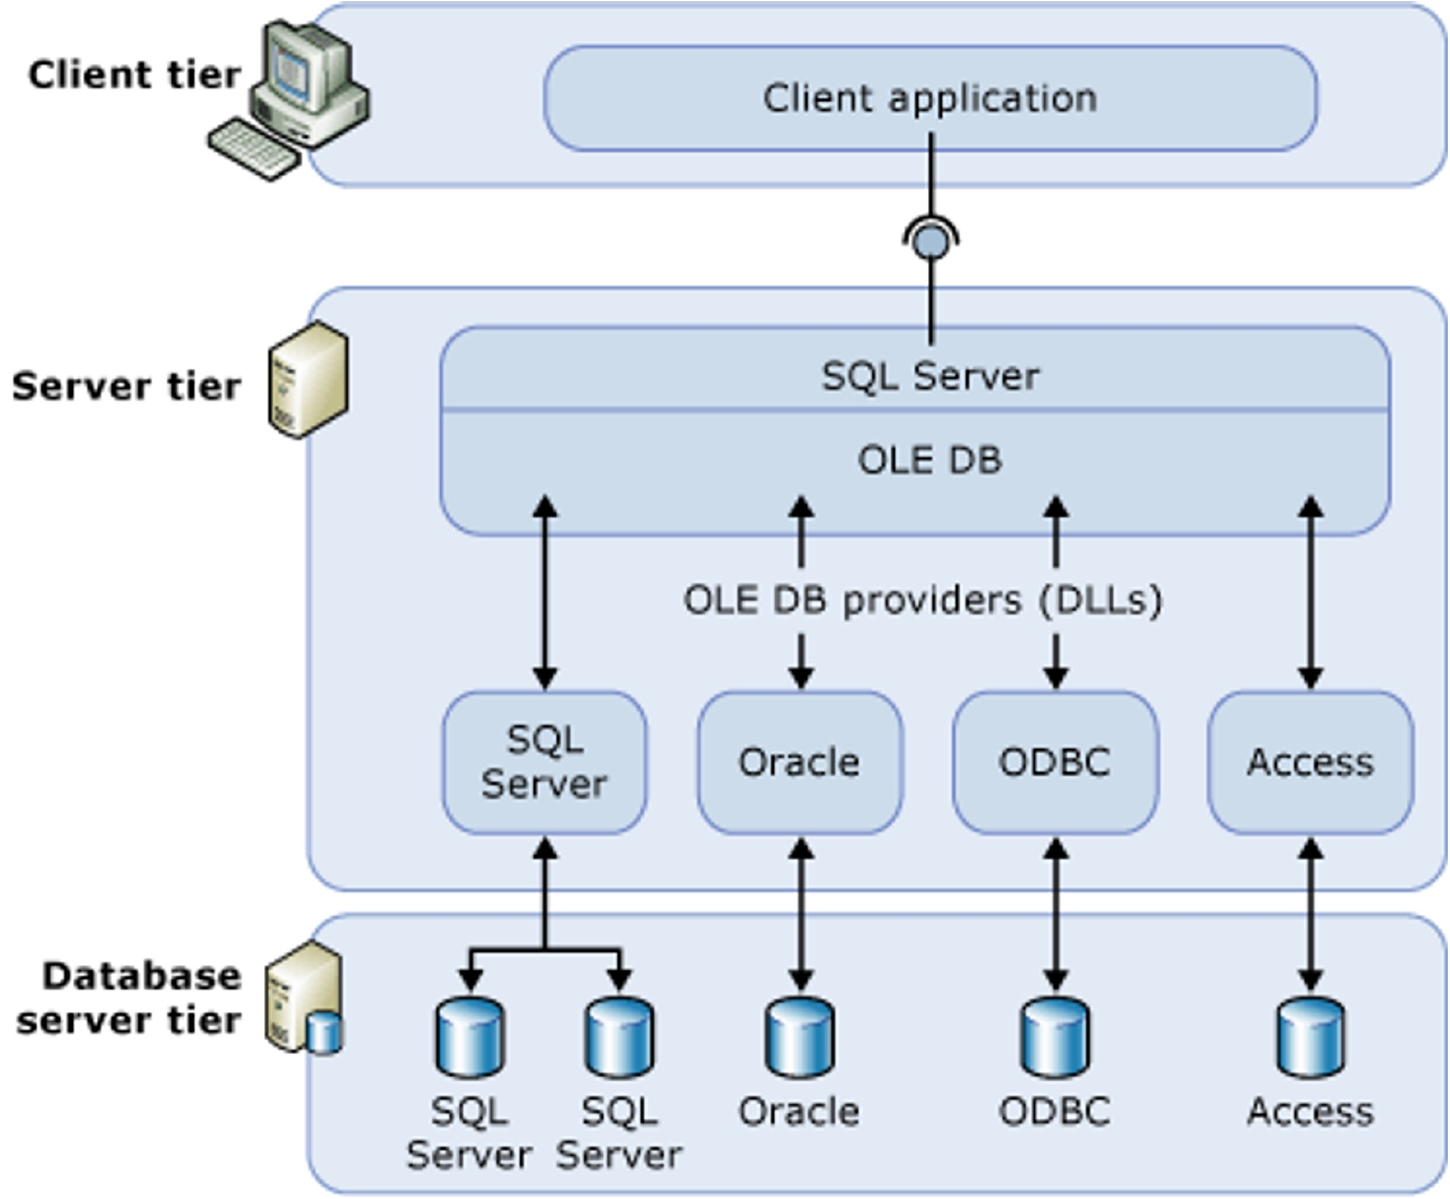
\includegraphics[width=0.8\linewidth]{img/linkedServer.png}
    \caption{Linked server architecture: SQL Server reaches heterogeneous sources (Oracle, Access, Excel, other SQL Server instances) through OLE DB providers.}
    \label{fig:linked-server-architecture}
\end{figure}

\subsubsection{Configuration}
\label{subsec:linked-server-config}

A linked server is created either through SSMS (Server Objects $\rightarrow$ Linked Servers $\rightarrow$ New) or with T-SQL:

\begin{lstlisting}
EXEC sp_addlinkedserver
    @server = 'ORACLE_SALES',
    @srvproduct = 'Oracle',
    @provider = 'OraOLEDB.Oracle',
    @datasrc = 'sales.example.com/ORCL';

EXEC sp_addlinkedsrvlogin
    @rmtsrvname = 'ORACLE_SALES',
    @useself = 'FALSE',
    @rmtuser = 'report_user',
    @rmtpassword = 'password';
\end{lstlisting}

\subsubsection{Distributed Queries}
\label{subsec:distributed-queries}

Remote objects are referenced with the four-part notation:

\begin{center}
\texttt{linked\_server.database.schema.object}
\end{center}

\begin{lstlisting}
-- Join between local and remote table (Oracle)
SELECT l.customer_id, l.name, r.total_orders
FROM dbo.customers AS l
JOIN ORACLE_SALES.sales.dbo.order_summary AS r
    ON l.customer_id = r.customer_id;

-- Compare data between two servers for data quality
SELECT *
FROM LOCAL_CRM.crm.dbo.contacts AS A
JOIN ORACLE_LEGACY.legacy.dbo.contacts AS B
    ON A.email = B.email
WHERE A.phone <> B.phone;  -- Discrepancies in phone numbers
\end{lstlisting}

\begin{notebox}
\textbf{Performance.}
Distributed queries can be slow when the query optimizer fails to push filters down to the remote server. Check the execution plan and consider \texttt{OPENQUERY} to force remote execution:
\begin{lstlisting}
SELECT * FROM OPENQUERY(ORACLE_SALES,
    'SELECT * FROM orders WHERE order_date > SYSDATE - 30');
\end{lstlisting}
\end{notebox}

\subsection{Connecting to SQL Server}
\label{sec:sql-server-connection}

\subsubsection{SSMS Configuration}
\label{subsec:ssms-connection}

At startup, SQL Server Management Studio's connection dialog asks for:

\begin{itemize}
    \item \textbf{Server type}: Database Engine (for the relational engine), Analysis Services, Integration Services, or Reporting Services.

    \item \textbf{Server name}: the instance name in the form \texttt{hostname} (default instance) or \texttt{hostname\textbackslash instance} (named instance). For Azure SQL: \texttt{server.database.windows.net}.

    \item \textbf{Authentication}:
    \begin{itemize}
        \item \textit{Windows Authentication}: uses the current Windows user's credentials (Kerberos/NTLM). It is preferable in Active Directory environments.
        \item \textit{SQL Server Authentication}: a login and password stored in SQL Server. It requires the instance to be configured in mixed mode.
        \item \textit{Azure Active Directory}: for Azure SQL databases with cloud identities.
    \end{itemize}
\end{itemize}

\subsubsection{Connection String for Applications}
\label{subsec:connection-strings}

Applications connect through a connection string (see also Section~\ref{subsec:pyodbc-connection}):

\begin{lstlisting}[language={}, basicstyle=\ttfamily\scriptsize]
-- SQL Server Authentication
Server=myserver.example.com;Database=sales;
User Id=app_user;Password=secret;

-- Windows Authentication
Server=myserver.example.com;Database=sales;
Trusted_Connection=True;

-- Azure SQL
Server=myserver.database.windows.net;Database=sales;
User Id=app_user;Password=secret;Encrypt=True;
\end{lstlisting}
